\section{Emergent Behaviours}

\subsection{Different Graph Topologies}

The rewiring algorithm \cite{aamas2010} was ran on graphs with a random topology, such as those graphs generated by the Erdos-Renyi generator.
We ran our implementation of this rewiring algorithm on scale-free and small-world graphs.
Scale-free and small-world graphs are a better representation of social networks than random graphs.
In social networks, each user is likely to belong to one or more cliques.
Large numbers of the users in a clique are likely to be connected.
This clique nature creates a number of clusters in the topology, which is different from random topologies where clusters are uncommon.

When we ran these same algorithms on the scale-free and small-world graphs, generated randomly using the JUNG Barab\'{a}si-Albert and Kleinberg Small-world generators, we found that the donation rate remained at a similar level.
Our results show that there is no significant effect on the donation rate with different graph topologies.
Figure \ref{fig:donation-rates-scale-and-small-world} shows as an example, the average donation rates observed on random, scale-free, and small-world graphs against average degree.
The results in this graph used a population size of 200 agents and employed the individual replace worst rewiring strategy, however we found similar behaviour exhibited in all our tests.

\begin{figure}[htbp]
	\centering
	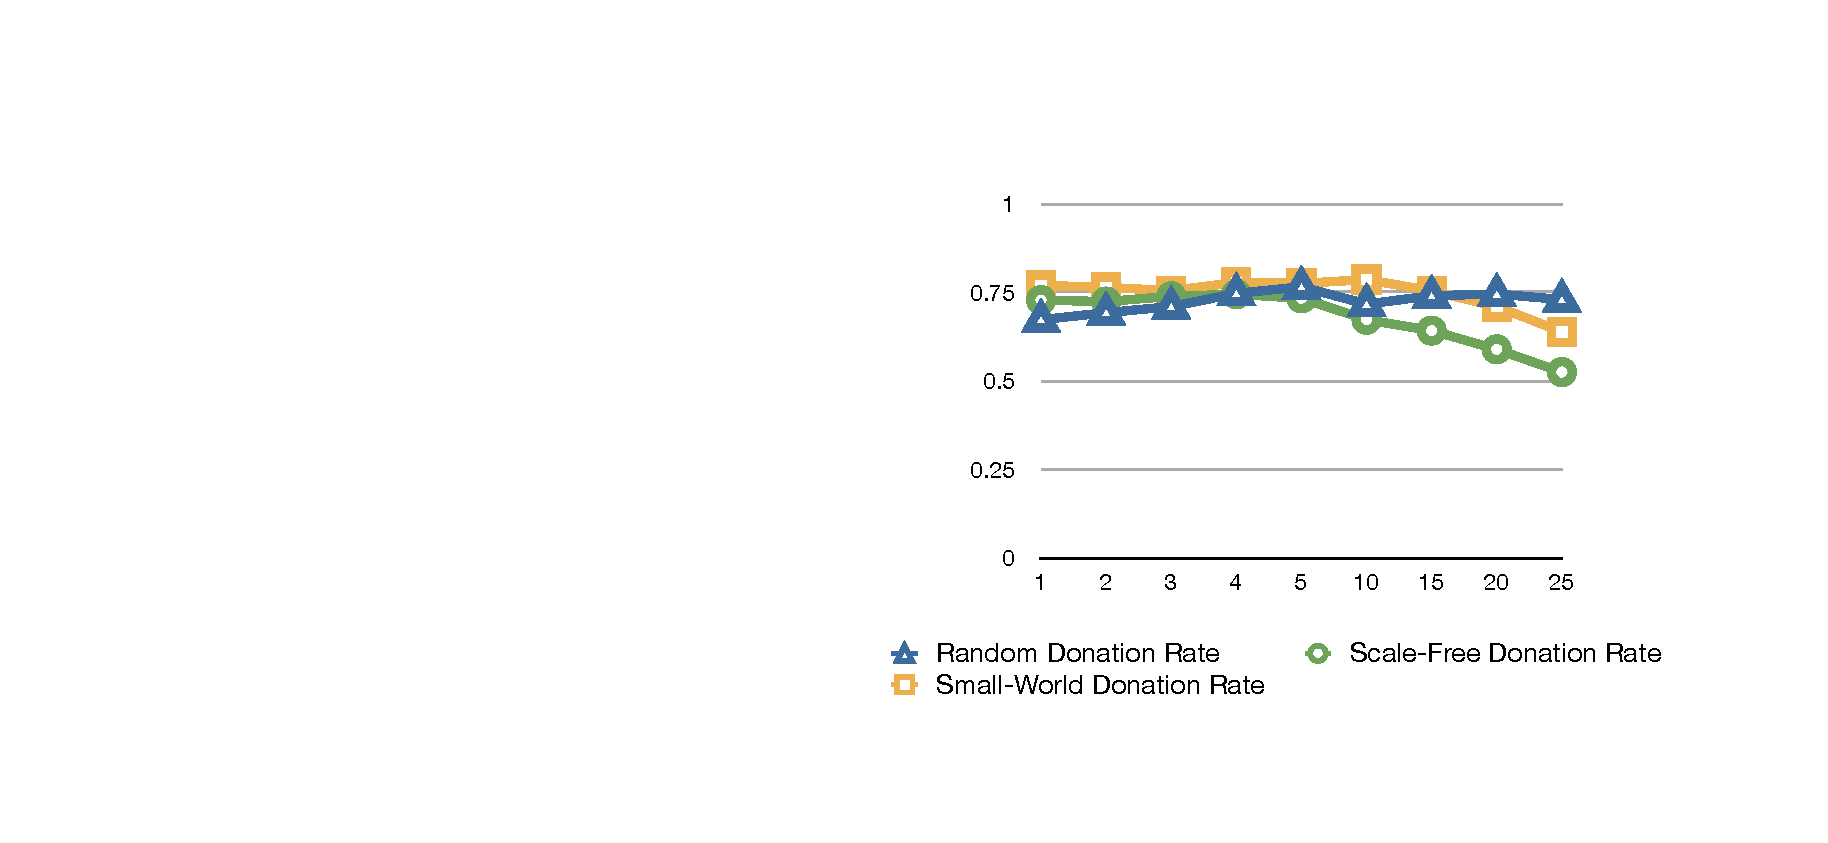
\includegraphics[width=0.7\linewidth]{img/small_world_scale_free_donation_rates.pdf}
	\caption{Donation rates against average degree}
	\label{fig:donation-rates-scale-and-small-world}
\end{figure}

We examined the topological changes caused by the rewiring of the graphs and noticed that although the initial topology was small-world and scale-free, the rewiring caused the topology to morph into a graph with a random topology within just a few generations.

\subsection{Retaining Initial Topological Nature}

We decided that we should look at preserving the initial topological nature of the graphs throughout the simulation, so we decided to look at alternative methods of rewiring that could manage to maintain a similar topology but preserve a donation rate as high as the current rewiring algorithms.

To this end, we decided to create an algorithm that attempts to maintain the same number of small-world connections and long-distance connections during the rewiring. This was achieved by measuring the shortest path lengths when removing connections  and attempting to forge connections to neighbours with a similar shortest path length when rewiring an agents neighbourhood.

We created two algorithms, the first was based on the random rewiring strategy and was designed in order to test how the topology changes over time. This differs from the random rewiring strategy in two ways:
\begin{itemize}
	\item After agent A removes agent B from its neighbourhood, the shortest path length between these two nodes is measured (length AB).
	\item When a randomly selected agent (C) is chosen to replace agent B in agent A's neighbourhood, the shortest path length between agent A and agent C is measured (length AC). Agent C will only be added to agent A's neighbourhood if the lengths AB and AC are similar. In the case that these lengths are different, then this is repeated with a different, randomly selected agent C.
\end{itemize}

The second rewiring algorithm is based on the group replace worst rewiring algorithm.
Like the above algorithm, when a neighbour is removed, the shortest path length between the two agents is measured.
The group replace worst algorithm is used to suggest new neighbours, but these neighbours will only be added if the shortest path length is similar to the path that was removed. Any discrepancy in the number of neighbours added and the number of neighbours removed will be made up for by adding neighbours randomly, in a similar fashion to the algorithm above.

The results in figure \ref{fig:new_rewiring_results} show the impact that these new rewiring algorithms have on the donation rate. It can be seen in these graphs that the new donation rate for the random algorithm performs similarly to that of the existing random rewire algorithms. It can also been seen that the algorithm based on the group replace worst also exhibits similar behaviour to that of the existing group replace worst algorithm.
We found that the new rewiring algorithm based on the group replace worst rewiring algorithm manages to maintain the same small-world nature of the initial graphs.

\begin{figure}[htbp]
	\centering
	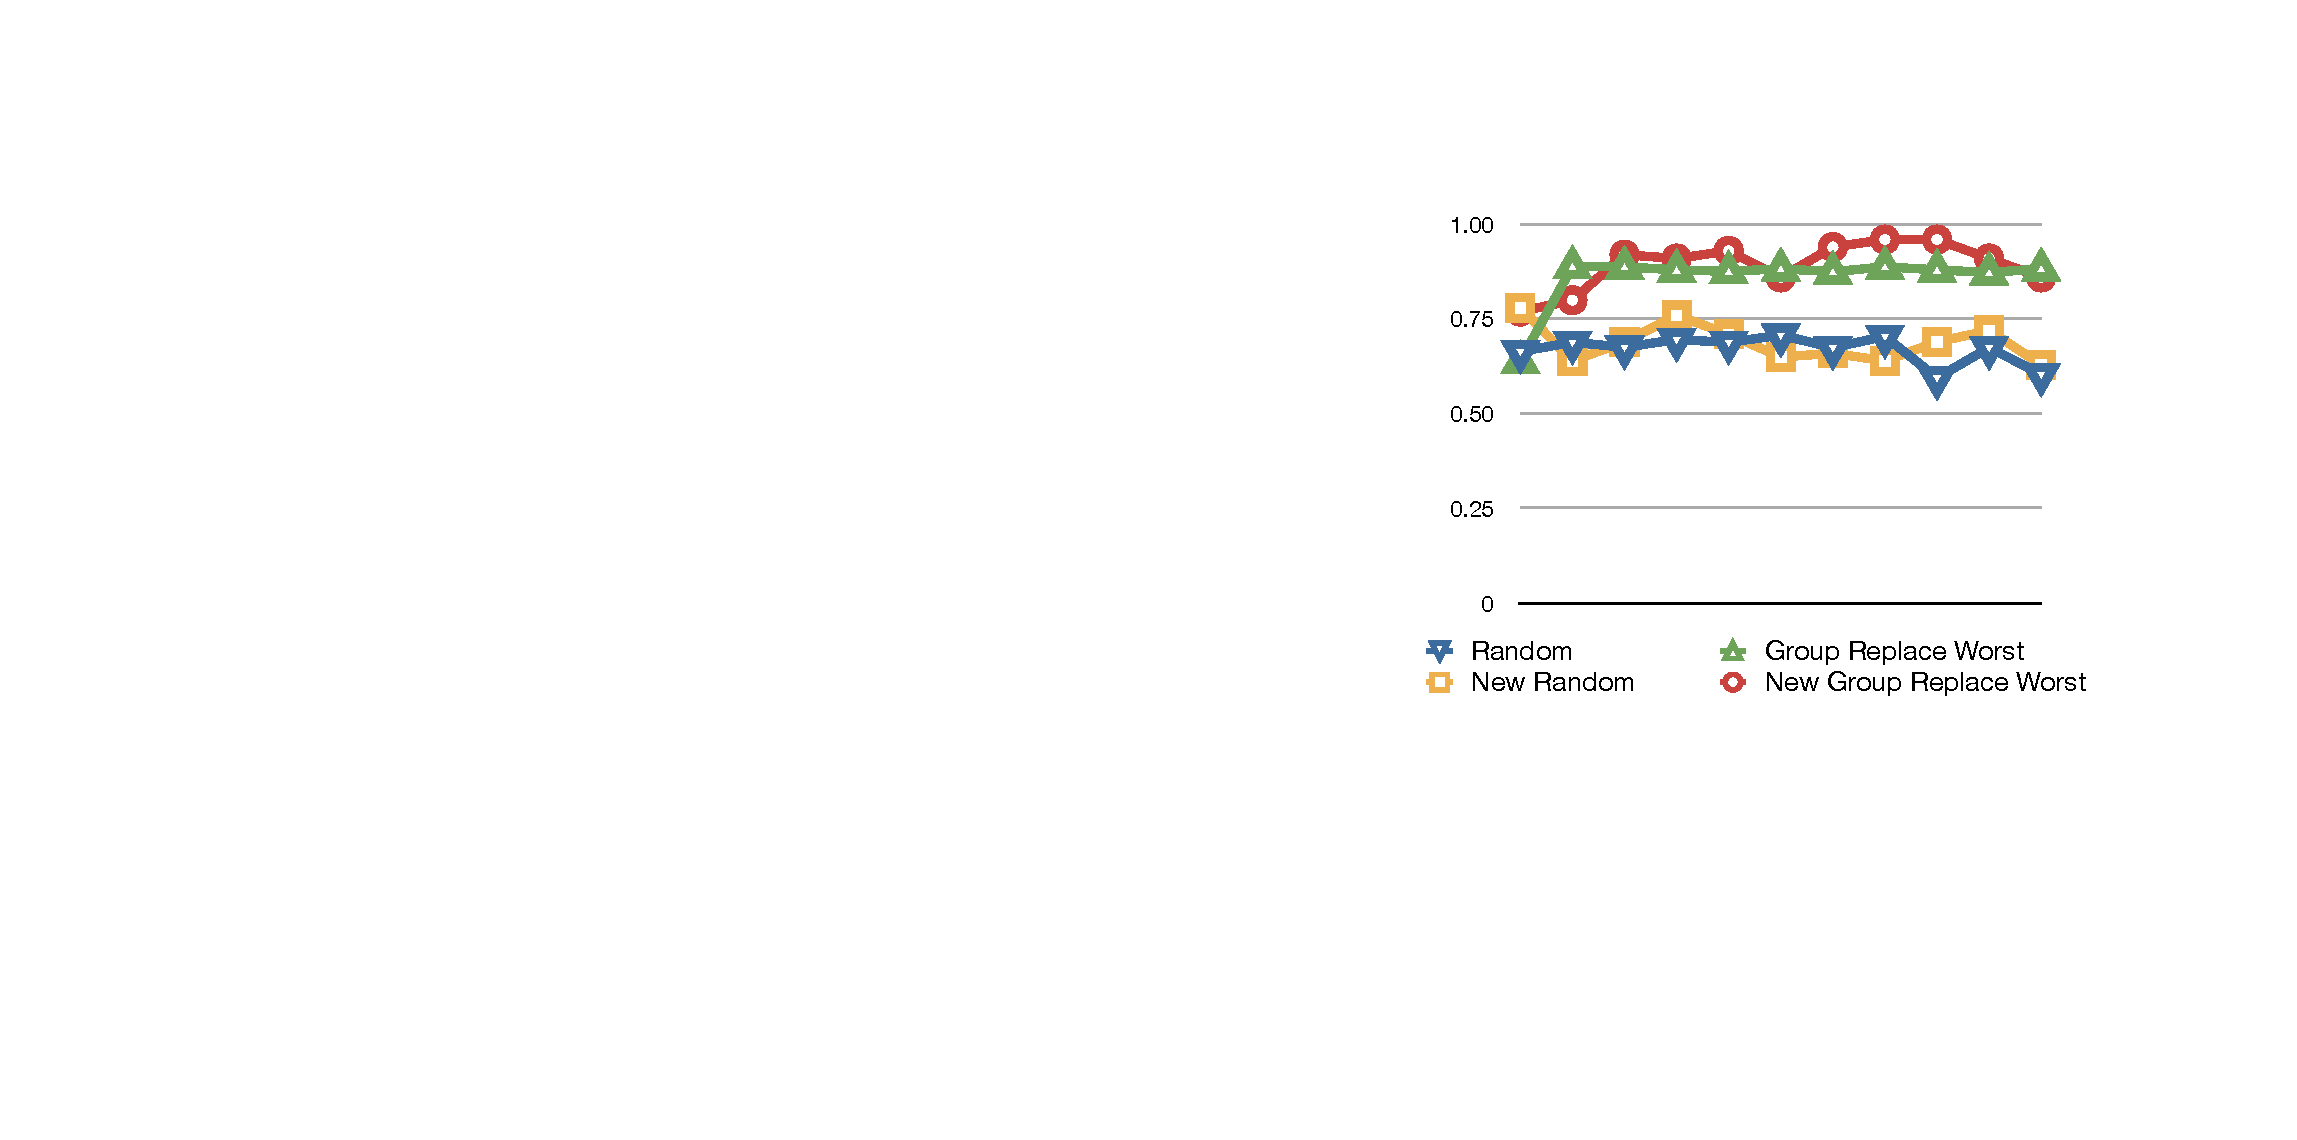
\includegraphics[width=0.7\linewidth]{img/new_rewiring_results.pdf}
	\caption{Donation rates for new rewiring strategies}
	\label{fig:new_rewiring_results}
\end{figure}